\paragraph{Objectives of the CALREC subproject.}

\begin{figure}
\begin{center}
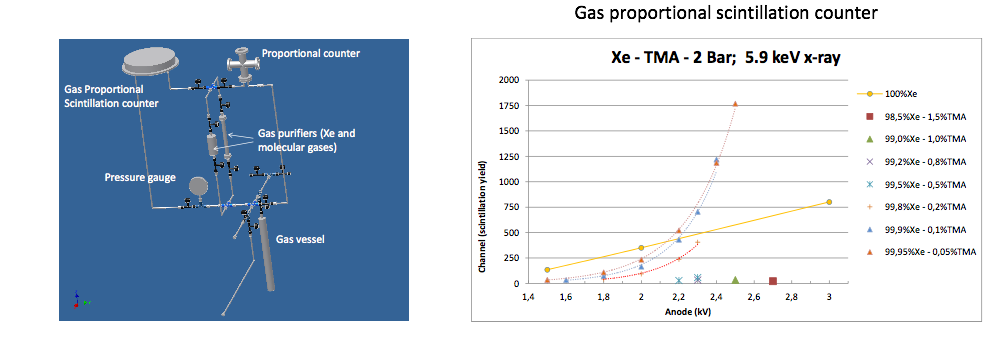
\includegraphics[width=0.99\textwidth]{img/TMA.png}
%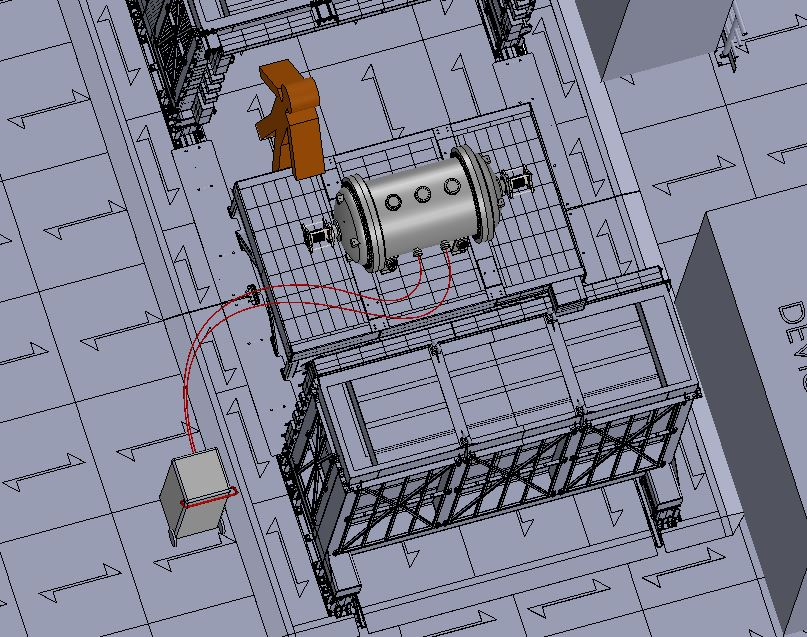
\includegraphics{img/CALIB_LSC_sources.jpg}
\caption{\small Left. A small experimental setup to test gas mixtures. Right: initial results obtained with the setup, showing that very small concentrations of TMA result in a very large increase of the scintillation yield. Larger concentrations, on the other hand, quench the yield. }
\label{fig:additives}
\end{center}
\end{figure}

The specific objectives of this subproject are:
\begin{enumerate}
\item {\bf Photo-detectors calibration system}. Design, construction, commissioning and operation of a calibration system to estimate the gain and noise of the SiPMs and PMTs sensors of the tracking plane and energy plane of NEW and NEXT-100. 

\item {\bf Energy calibration system}. Design, construction, commissioning and operation of an energy calibration system with external radioactive sources for NEW and NEXT-100.

\item {\bf Position calibration system}. Design, construction, commissioning and operation of a position calibration system using the X-rays produced by a $^{83}$Rb source. 

\item {\bf Xenon additives}. Development of a dedicated testing system to evaluate additives capable to improve the performance of pure xenon. 

\end{enumerate}

